%\documentclass[11pt]{article}
%\usepackage{beamerarticle}
%\usepackage{graphicx}
\documentclass[12pt,xcolor=dvipsnames%,handout
]{beamer}
\PassOptionsToClass{beamer}{handout}
\usepackage{pgfpages} 
\pgfpagesuselayout{4 on 1}[letterpaper,landscape,border shrink=3mm]
\usepackage{amsmath}
\usepackage{helvet}
\usepackage{mymacros}
\usepackage{xspace}
\usepackage{pifont}
\usepackage[all,cmtip,arrow]{xy}  %for xy-pic fonts
%%macs
%For this presentation, I don't want citations
\renewcommand{\cite}[1]{\relax}
\newcommand{\V}{\ensuremath{\mathcal V}\xspace}
\newcommand{\mbold}[1]{\ensuremath{\mathbf{#1}}\xspace}
\makecs{\mbold}{ABDP}
\newcommand{\exmpl}[1]{{\color{green!50!black} #1}}
\newcommand{\dsize}{\displaystyle}
\DeclareMathOperator{\End}{End}
\DeclareMathOperator{\Var}{Var}
\DeclareMathOperator{\Cg}{Cg}
\DeclareMathOperator{\Sub}{Sub}
\DeclareMathOperator{\Con}{Con}
\DeclareMathOperator{\Rel}{Rel}
\newcommand{\bigpause}{\pause\bigskip}
\DeclareMathOperator{\CSP}{CSP}
\newcommand{\FF}{\mathbb{F}}
\DeclareMathOperator{\Pol}{Pol}
\DeclareMathOperator{\Inv}{Inv}
\renewcommand{\.}{\cdot}
\DeclareMathOperator{\core}{core}
\newcommand{\reduc}{\leq_{\text{\textnormal{p}}}}
\newcommand{\equivp}{\equiv_{\text{\textnormal{p}}}}
\newcommand{\NP}{\ensuremath{\mathbb{NP}}\xspace}
\renewcommand{\P}{\ensuremath{\mathbb{P}}\xspace}
\newcommand{\Blue}{\textcolor{blue!50!black}}
\newcommand{\Red}{\textcolor{violet!50!red}}
\newcommand{\Green}{\textcolor{green!55!black}}
\let\origemph=\emph 
\let\origtextbf=\textbf 
%%endmacs
%%
\parskip=10pt
%% Beamer Setup
\mode<handout>{\beamertemplatesolidbackgroundcolor{black!5}}
\mode<presentation>{
  \usetheme{Singapore}
  \usetheme{Frankfurt}
%  \useinnertheme[shadow]{rounded}
  \setbeamertemplate{navigation symbols}[only frame symbol]{}
}
\mode<beamer>
{%
  \let\emph=\alert
  \renewcommand{\textbf}[1]{{\usebeamercolor[fg]{example text}%
     \origtextbf{#1}}}
}
\mode<article>{\usepackage{fullpage}}
%%
%\title{\TeX\ and \LaTeX\ in the Mathematics Department}
%\author{Clifford Bergman}
\setbeamertemplate{headline}{\scriptsize{\vspace*{0.3cm}\hspace*{0.3cm}\insertframenumber}} 

\begin{document}
\title{Constraint Satisfaction Problems,\\Graph Theory,\\and Universal Algebra}
\author{Cliff Bergman}
\frame[plain]{\titlepage}

\begin{frame}
\frametitle{What is a CSP?}

  Informally, a \textbf{C}onstraint \textbf Satisfaction \textbf Problem
  consists of
  \begin{itemize}
  \item a list of variables ranging over a finite domain and
  \item a set of constraints on those variables.
  \end{itemize}

  \textbf{Problem:} can we assign values to all the variables so that
  all of the constraints are satisfied?

\end{frame}

\begin{frame}
  \frametitle{Examples}

A system of linear equations is a CSP
\begin{alignat*}4
  a_{11}x_1 &&+ a_{12}x_2 &&+ \cdots &&+ a_{1n}x_n &= b_1 \\
  a_{21}x_1 &&+ a_{22}x_2 &&+ \cdots &&+ a_{2n}x_n &= b_2 \\
  &&\;\vdots \\
  a_{m1}x_1 &&+ a_{m2}x_2 &&+ \cdots &&+ a_{mn}x_n &= b_m \\
\end{alignat*}
\end{frame}

\begin{frame}
  Also, a system of nonlinear equations is a CSP
\begin{alignat*}4
  a_{11}x_1^2x_3 &+ a_{12}x_2x_3x_7 &&+ \cdots &&+ a_{1n}x_4x_n^3 &&= b_1 \\
  a_{21}x_2x_5 &+ a_{22}x_2 &&+ \cdots &&+ a_{2n}x_4^3 &&= b_2 \\
 &&&\vdots \\
  a_{m1}x_3x_5x_8 &+ a_{m2}x_2 &&+ \cdots &&+ a_{mn}x_n &&= b_m \\
\end{alignat*}
\end{frame}

\begin{frame}
  For a fixed $k$, determining whether a graph is $k$-colorable is a CSP
  \begin{center}
    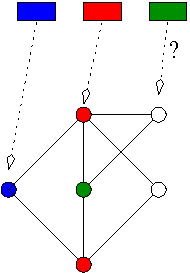
\includegraphics{k-col}
%    \fbox{picture suggesting 3-colorability}
  \end{center}
\end{frame}


\begin{frame}
Given a propositional formula $\phi(x_1,\dots,x_n)$, determine whether $\phi$ is satisfiable
\bigskip
\begin{equation*}
\phi(x,y,z) = (x\join y \join z') \meet (x'\join y \join z')
\end{equation*}
then 
\begin{equation*}
\phi(0,0,1) = 1
\end{equation*}
\end{frame}

\begin{frame}
  \frametitle{Algorithms}
  There is an efficient algorithm (Gaussian elimination) for solving any
  linear system.
  That is

\setbeamercolor{block body example}%
{parent=normal text,use=block title example,bg=block title example.bg!25!bg}
  \begin{exampleblock}{}
    There is an algorithm that accepts as \emph{input} a linear system
    and decides whether that system has a solution.

    \smallskip
    The running time of the algorithm is bounded above by $f(s)$ where
    $f$ is a polynomial and $s$ is the size of the system.
  \end{exampleblock}
  \pause

  The particular system is an \emph{instance} of the \emph{problem}
  LINEAR SYSTEM
  
\end{frame}

\begin{frame}
  Similarly

  \setbeamercolor{block body example}%
  {parent=normal text,use=block title example,bg=block title example.bg!25!bg}
  \begin{exampleblock}{}
    There is an algorithm that accepts as input a graph and decides
    whether the graph is 2-colorable.

    \smallskip
    The running time is bounded by $f(s)$ where $f$ is a polynomial and
    $s$ is the size of the graph.
  \end{exampleblock}

  The graph is an instance of the problem 2-COLORABILITY.
\end{frame}

\begin{frame}
\setbeamercolor{block body example}%
  {parent=normal text,use=block title example,bg=block title example.bg!25!bg}
  \begin{exampleblock}{}
  There is an algorithm that accepts as input a formula, $\phi = \phi_1 \meet \phi_2 \meet \cdots \meet \phi_k$, in which each $\phi_i$ is bijunctive, and decides whether $\phi$ is satisfiable.
  
  \smallskip
  the running time is bounded by $f(k)$ in which $f$ is a polynomial
  \end{exampleblock}
  
  $\phi$ is an instance of the problem 2-SAT.

\bigpause
  We say these algorithms run in \emph{polynomial time}.
\end{frame}

\begin{frame}
  No polynomial-time algorithm is known for, NONLINEAR SYSTEM,
  3-COLORABILITY, or 3-SAT.

  \bigpause
  However, any candidate solution to either of these problems can be
  checked in polynomial-time. 

  \bigpause
  Thus these problems are solvable in \emph{nondeterministic polynomial
    time.} 
\end{frame}

\begin{frame}
  Let $X$ and $Y$ be two problems. We write $X \reduc Y$ to indicate that
  $Y$ is at least as hard as $X$.

  \bigpause
  Somewhat more precisely: any algorithm for solving $Y$ can be
  transformed into an algorithm for $X$ without drastically increasing
  its running time.

  \bigpause
  It is possible for $X\reduc Y \reduc X$. In that case, write $X\equivp
  Y$. 

\end{frame}

\begin{frame}
  \P is the class of all problems solvable in polynomial time. Its
  members are called \emph{tractable.}

  \NP is the class of problems solvable in nondeterministic polynomial
  time. 

  \pause
  \begin{itemize}
  \item $\P \sseq \NP$
  \item Both $\P$ and $\NP$ are downsets, i.e., \\
    $Y\in \P \mathrel{\&} X\reduc Y \implies X\in \P$
  \end{itemize}

  \pause
  The maximal members of \NP are called \emph{\NP-complete.} 

  
  3-COLORABILITY, NONLINEAR SYSTEM, and 3-SAT are known to be
  \NP-complete. 
\end{frame}

\begin{frame}
  \frametitle{\$$2^{20}$ question: $\P \overset{?}{=} \NP$.}

  \pause
  If $\P=\NP$ then all of the above distinctions go away. Almost every
  problem that mathematicians actually care about can be solved
  efficiently. Just build bigger computers.

  \pause
  In particular, this talk becomes pointless. So assume $\P\neq \NP$.

  \pause
  \begin{theorem}[Ladner, 1975 \cite{Ladner1975}]
    If $\P \neq \NP$ then there are problems in $\NP-
    \P$ that are not \NP-complete.
  \end{theorem}

\end{frame}

\begin{frame}
  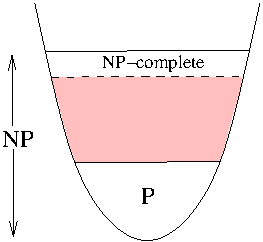
\includegraphics[scale=1.25]{complexity}
  \qquad
  \parbox[b][2in][c]{1.5in}{If $\P\neq \NP$ then the pink area is nonempty.}
\end{frame}

\begin{frame}
  \frametitle{Formal Definition of CSP}

  Let $D$ be a set, $n$ a positive integer\\
  An \emph{$n$-ary relation on $D$} is a subset of $D^n$

  \pause
  $\Rel_n(D)$ denotes the set of all $n$-ary relations on $D$

  $\Rel(D) = \bigcup\limits_{n>0} \Rel_n(D)$
\end{frame}

\begin{frame}
  Let $D$ be a finite set and $\Delta\sseq \Rel(D)$

  $\CSP(\<D,\Delta\>)$ is the problem:\\
  \textbf{instance:} A finite set $V=\setof{v_1,\dots,v_n}$ of
    \emph{variables}
    and\\
    a finite set $\setof{C_1,\dots,C_m}$ of \emph{constraints}

    Each constraint $C_i$ is a pair $(\seqof{x_{i1},\dots,x_{i\,p_i}},\,
    \delta_i)$ in which $x_{i1},\dots,x_{i\,p_i} \in V$ and $\delta_i\in
    \Delta$

    \pause
    \textbf{Question:} Does there exist a mapping $f\colon V\to D$ such
    that for all $i\leq m$, $\<f(x_{i1}),\dots,f(x_{i\,p})\>\in \delta_i$?

    \pause
    $\CSP(\<D,\Delta\>)$ always lies in \NP.

%    $\CSP\<D,\Delta\>$ is \emph{finitary} if $\Delta$ is finite. 
\end{frame}

\begin{frame}
  \frametitle{Example: Linear Equations over $\FF_2$}

  $D=\{0,1\}$ \\
  $\Delta$ consists of all relations
  \begin{equation*}
    \delta_{n,\mathbf a}^b = \bigl\{\,\<x_1,\dots,x_n\>\in D^n :
      a_1x_1+\cdots a_nx_n = b\bigr\}
  \end{equation*}
Here, $\mathbf a= \<a_1,a_2,\dots,a_n\>\in D^n$, $b\in D$.

\bigskip
  Then $\CSP(\<D,\Delta\>)$ is LINEAR SYSTEM
\end{frame}

\begin{frame}
  \frametitle{Example: 3-colorability}

  $D=\{\Red{r},\Green{g},\Blue{b}\}$, \quad $\Delta=\{\kappa_3\}$\\
  $\kappa_3=\setof{(x,y)\in D : x\neq y}$

  Then $\CSP(\<D,\Delta\>)$ is the 3-colorability problem

  \bigskip

    \begin{columns}
      \begin{column}{1.5in}
        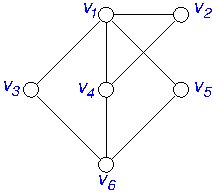
\includegraphics{col_csp}
      \end{column}
      \begin{column}{2in}
        $V=\{v_1,\dots,v_6\}$\\
        $\<v_1,v_2\>\in \kappa$\\
        $\<v_1,v_3\>\in \kappa$\\
        $\<v_1,v_4\>\in \kappa$\\
        $\<v_2,v_4\>\in \kappa$\\
        \qquad$\vdots$\\
        $\<v_5,v_6\>\in \kappa$
      \end{column}
    \end{columns}
  \end{frame}

\begin{frame}
\frametitle{Example: 2-SAT}
$D=\{0,1\}$\\
For a bijunctive clause $\phi(x,y)$, 
\begin{equation*}
\delta_\phi= \setof{\<a,b\>\in D^2: \phi(a,b)=1}
\end{equation*}

\pause
\begin{tabular}{cc|c}
 $x$ & $y$ &$x\join y'$  \\
 \hline
0 & 0 & 1\\
\visible<2>{0 & 1 & 0}\\
1 & 0 & 1\\
1 & 1 & 1
\end{tabular}
\uncover<3->{\qquad \parbox{2.5in}{So $\delta_{x\join y'} = \{\<00\>,\,\<10\>,\,\<11\>\}%=\\ \{0,1\}^2-\{\<01\>\}
$}}

\bigskip
\uncover<4->{$\displaystyle\Delta=\{\delta_{x\join y},\, \delta_{x\join y'},\,\delta_{x'\join y},\, \delta_{x'\join y'}\}$}
\end{frame}

\begin{frame}
\frametitle{Example: Horn-SAT}
\emph{Horn formula:}\\
 $(x_0 \meet x_1 \meet \cdots \meet x_{i-1} \meet x_{i+1} \meet \cdots \meet x_{n-1}) \rightarrow x_i$\\[6pt]
\emph{Equivalently:}\\
 $x_0' \join x_1' \join \dots x_{i-1}' \join x_i \join \cdots \join x_{n-1}'$

\bigpause
Corresponding relation $\gamma^n_i = \{0,1\}^n-\{\<111\dots0\dots111\>\}$

\bigpause
Horn-SAT is $\CSP\<D,\Gamma\>$\\
$D=\{0,1\}$,\quad $\Gamma=\setof{\gamma^n_i : 0\leq i <n}$
\end{frame}

\begin{frame}
  \frametitle{Schaefer's Dichotomy}

  \begin{theorem}[Schaefer, 1978 \cite{Schaefer1978}]
    Let $D=\{0,1\}$. There are six families $\Delta_0,
  \dots, \Delta_5$ such that
  \begin{equation*}
    \CSP(\<D,\Delta\>) \in \P \iff \Delta \sseq \Delta_i, \text{some $i< 6$}
  \end{equation*}
  Otherwise $\CSP(\<D,\Delta\>)$ is $\NP$-complete.
\end{theorem}
\end{frame}

\begin{frame}
{\large The six families}
$\Delta_0 = \setof{\delta : \<0,0,\dots,0\>\in \delta}$ (``All False'')\\[2pt]
$\Delta_1 = \setof{\delta : \<1,1,\dots,1\>\in \delta}$ (``All True'')\\[2pt]
$\Delta_2 = \{\delta_{x\join y},\, \delta_{x\join y'},\,\delta_{x'\join y},\, \delta_{x'\join y'}\}$ (bijunctive)\\[2pt]
$\Delta_3 = \Gamma$ (Horn)\\[2pt]
$\Delta_4 = \Gamma^\partial$ (dual-Horn)\\[2pt]
$\Delta_5$ (affine, i.e., linear system over $\FF_2$)
\end{frame}

\begin{frame}
  \frametitle{Two Motivating Questions}

  \begin{enumerate}
  \item \emph{Dichotomy Conjecture}\\ Every $\CSP(\<D,\Delta\>)$ either
    lies in \P\ or is $\NP$-complete.

    \pause

  \item \emph{Tractability Problem}\\ Characterize those CSPs that lie in \P.
  \end{enumerate}
  
  \pause
  What would a characterization look like? What language could we use?
\end{frame}

\begin{frame}
\frametitle{Why is 2-SAT tractable, but 3-SAT is not?}

2-SAT: $\Delta_2=\{\delta_{x\join y},\,\delta_{x\join y'},\, \delta_{x'\join y},\, \delta_{x'\join y'}\} $

\smallskip
3-SAT: $\Lambda=\{\lambda_0,\lambda_1,\dots, \lambda_7\}$

\pause
\begin{equation*}
M(x,y,z) = \begin{cases}
	0 \quad&\text{if at least 2 of $x,y,z$ equal 0}\\
	1 &\text{otherwise}
	\end{cases}
\end{equation*}
``Majority Operation''

\pause
$M$ preserves each $\delta\in \Delta_2$:
\begin{equation*}
\begin{matrix}
\<a_1, &b_1\> &\in \delta\\
\<a_2, &b_2\> &\in \delta\\
\<a_3, &b_3\> &\in \delta \text{ implies}\\
\<M(a_1,a_2,a_3), &M(b_1,b_2,b_3)\> &\in \delta
\end{matrix}
\end{equation*}

\end{frame}

\begin{frame}
But $M$ fails to preserve each $\lambda\in \Lambda$

\medskip
For example, with $\lambda=\lambda_{x\join y\join z'}=\{0,1\}^3-\{\<001\>\}$ 

\begin{align*}
\<1,0,0\> &\in \lambda\\
\<0,0,1\> &\in \lambda\\
\<0,1,1\> &\in \lambda \text{ but}\\
\<0,0,1\> &\notin \lambda
\end{align*}

\end{frame}

\begin{frame}
  \frametitle{Polymorphisms}

  \begin{definition}
    Let $\delta \in \Rel_k(D)$ and $f\: D^n \to D$. We say 
    \emph{$f$ preserves $\delta$} if
    \begin{equation*}
      \begin{split}
        (a_{11}, \dots, a_{1k}),&\dots, (a_{n1},\dots, a_{nk}) \in
        \delta \implies\\ 
        &\bigl( f(a_{11},\dots, a_{n1}), \dots, f(a_{1k},\dots,a_{nk})
        \bigr) \in \delta
    \end{split}
    \end{equation*}

  \end{definition}

  \begin{overprint}
  \onslide<2|handout:0>
  $f$ is an \emph{$n$-ary operation} on $D$.
  % 
  \onslide<3|handout:1>
    \begin{equation*}
      \newcommand\flab{\scriptstyle{f}}
      \begin{matrix} a_{11} & a_{12} & \dots & a_{1k} & \in & \delta \\
        a_{21} & a_{22} & \dots & a_{2k} & \in & \delta \\
        \vdots  & \vdots &       &\vdots  &     & \vdots \\
        a_{n1} & a_{n2} & \dots & a_{nk} & \in & \delta \\
        \downarrow\flab &\downarrow\flab &  & \downarrow\flab \\
        \star  & \star  & \dots & \star  & \in & \delta
      \end{matrix}
    \end{equation*}
  \end{overprint}
\end{frame}

\begin{frame}
  \begin{definition}
    Let $\Delta$ be a set of relations on $D$. Then
    \emph{$\Pol(\Delta)$} denotes the set of all operations preserving
    all members of $\Delta$. These are the \emph{polymorphisms} of
    $\Delta$. 

    \bigpause

    Let $F$ be a set of operations on $D$. Then \emph{$\Inv(F)$} denotes
    the set of all relations preserved by all operations in $F$.
  \end{definition}
  
  \bigpause
Important point: $\<D,\Pol(\Delta)\>$ is an algebraic structure

\end{frame}

\begin{frame}
  \begin{theorem}
    Let $\Gamma, \Delta \sseq \Rel(D)$. Then
    \begin{equation*}
      \Pol(\Gamma) \sseq \Pol(\Delta) \implies \CSP(\Delta) \reduc
      \CSP(\Gamma). 
    \end{equation*}
  \end{theorem}

\pause
Thus, the richer the algebraic structure, the easier the corresponding CSP
\end{frame}

\begin{frame}
Schaefer proved that on $D=\{0,1\}$, there are 4 key polymorphisms:

\begin{center}
$M(x,y,z)$ (majority)\\
$x\meet y$\\
$x\join y$\\
$P(x,y,z) =x\oplus y \oplus z = x-y+z$
\end{center}

\bigskip
$\<\{0,1\},\Delta\>$ is tractable iff one of these four is a polymorphism of $\Delta$

\bigpause
Unfortunately, things become much more complicated when $\card{D}>2$.
\end{frame}


\begin{frame}
  One can go back and forth between relational and algebraic structures

  \begin{center}
    \begin{tabular}{ccc}
      \origtextbf{Relational} & &\origtextbf{Algebraic}  \\
      $\<D,\Delta\>$ & $\longrightarrow$ & $\<D,\Pol(\Delta)\>$ \\[2pt]
      $\<D, \Inv(F)\>$ & $\longleftarrow$ &$\<D,F\>$
    \end{tabular}
  \end{center}

  $\CSP\<D,\Delta\> \equivp \CSP\<D,\Inv(\Pol(\Delta))\>$

  \bigpause
  Perhaps the expressive power of algebra can be used to classify CSPs.

  \end{frame}

\begin{frame}
For a set of relations, $\Delta$, on $D$, $\Inv\bigl(\Pol(\Delta)\bigr)$ coincides with the set of relations definable from $\Delta$ by a \emph{positive primitive formula}.

\pause
$\phi(x_1,\dots,x_n)=(\exists y_1)(\exists y_2)\cdots(\exists y_m)\bigl(\delta_1(z_{1_1},\dots,z_{1_k}) \meet \dots \meet \delta_t(z_{t_1},\dots,z_{t_j})\bigr)$

Here $\delta_1\dots,\delta_t \in \Delta$ and every $z_{i_j} \in \{x_1,\dots,x_n,y_1,\dots,y_m\}$
\end{frame}



\begin{frame}
  \frametitle{Algebraic Facts}

  Let \A\ and \B\ be algebras

  $\B \text{ a subalgebra of \A} \implies \CSP(\B) \reduc \CSP(\A)$.

  $\B \text{ a homomorphic image of \A}\implies \CSP(\B) \reduc
  \CSP(\A)$. 
  
  $\CSP(\A^n) \equivp \CSP(\A)$

\end{frame}


\begin{frame}
  \begin{theorem}[Bulatov, Jeavons, Krokhin, 2000
    \cite{BulatovKrokhinJeavons2000}]
    If $\<D,\Delta\>$ is a core and every polymorphism is essentially unary,
    then $\CSP(\Delta)$ is \NP-complete.
  \end{theorem}

  $f$ is \emph{essentially unary} if $f(x_1,\dots,x_n) = g(x_j)$ for
  some unary $g$ and some $j\leq n$.

 \pause
 \begin{corollary}
    3-COLORABILITY, NONLINEAR SYSTEM, and 3-SAT are \NP-complete.
  \end{corollary}
\end{frame}



\begin{frame}
 
  \textbf{Informal reformulation of the dichotomy conjecture}\\
  If \A\ has some
  kind of decent algebraic structure then $\CSP(\A) \in \P$ otherwise
  $\CSP(\A)$ is \NP-complete.
\end{frame}

\begin{frame}
  \begin{definition}
    Let $n>1$. An $n$-ary operation $f$ is called a \emph{weak
      near-unanimity operation} if 
       \begin{equation*}
       \begin{gathered}
       f(x,x,\dots,x) = x \text{ and}\\
    f(y,x,x,x,\dots,x) = f(x,y,x,x,\dots,x) = \cdots\\
    = f(x,x,\dots,x,y)
  \end{gathered}
  \end{equation*}
  \end{definition}
  
  Note: no essentially unary operation is WNU
\end{frame}

\begin{frame}
  \begin{theorem}[Bulatov, Larose, Z\'adori, McKenzie, Mar\'oti
    \cite{BulatovJeavonsKrokhin2005,LaroseZadori2003,%
    MarotiMcKenzie2008}]
    If $\Delta$ is a core and $\Pol(\Delta)$ has no WNU operation
    then $\CSP(\Delta)$ is \NP-complete.    
  \end{theorem}
\end{frame}


\begin{frame}
  \frametitle{Reformuated Dichotomy Conjecture}

  Let $\Delta$ be a core. Then $\CSP(\Delta)$ is tractable if and only
  if it has a WNU polymorphism. Otherwise, it is \NP-complete. 

  \bigskip
  \begin{overprint}
    \onslide<2|handout:0> \centering{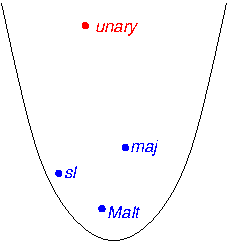
\includegraphics{dichotomy1}}
    \onslide<3|handout:0> \centering{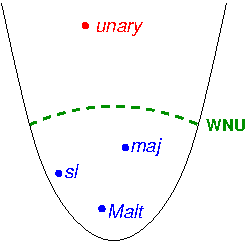
\includegraphics{dichotomy2}}
    \onslide<4|handout:0> \centering{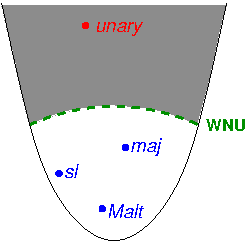
\includegraphics{dichotomy3}}
    \onslide<5-|handout:1>
    \begin{exampleblock}{Supporting Examples}
      \begin{itemize}
      \item 2-SAT, 2-COLARABILITY, LINEAR SYSTEM have a WNU.
      
             \item<6-> Let \A\ be an abelian group, $n=|A|$. Choose
        integers $k, l$ with $kl \equiv 1 \pmod n$. Then
        \begin{equation*}
          f(x_1,\dots,x_k) = l(x_1+\cdots + x_k)
        \end{equation*}
        is a WNU operation.
      \end{itemize}
    \end{exampleblock}
  \end{overprint}
\end{frame}

\begin{frame}
\frametitle{Two General Techniques for Tractable Algorithms}
%\begin{enumerate}
\begin{exampleblock}{Method 1}
If $\Pol(\Delta)$ contains a ``cube operation'' then $\CSP(\Delta)\in \P$
%\end{enumerate}
\end{exampleblock}

\pause
Examples of cube operations: 

$P(x,y,z) = x-y+z$\\
$M(x,y,z) = \text{majority}$

Essentially a generalization of Gaussian elimination. 

Algebras with a cube operation possess ``few subpowers''. This algebraic property is used to prove that the algorithm terminates in polynomial time.

\end{frame}

\begin{frame}
\begin{exampleblock}{Method 2}
If $\Pol(\Delta)$ contains WNU operations $v(x,y,z)$ and $w(x,y,z,u)$ satisfying $v(y,x,x)= w(y,x,x,x)$, then $\CSP(\Delta)\in \P$.
\end{exampleblock}

\pause
Examples: majority, semilattice 

Algebras with these operations have a property called ``congruence meet-semidistributivity.'' 

\end{frame}

\begin{frame}
\frametitle{Current State of Affairs}
The two general techniques do not cover all cases of a WNU. What to do next? 

\medskip
Two possible directions:
\begin{enumerate}
\item Find a completely new algorithm.
\item Combine the two existing algorithms.
\end{enumerate}

I am exploring the second approach.
\end{frame}


\end{document}





%%% Local Variables: 
%%% mode: latex
%%% TeX-master: t
%%% End: 
